\titre{}
\theme{Calcul différentiel}
\auteur{Nathan Scheinmann}
\niveau{3M}
\source{}
\type{serie}
\piments{}
\pts{}
\annee{2526}

\contenu{
	\tcblower
	On donne le graphe d'une fonction $f$. Esquisser le graphe de $f'$.
% Écrivez l'énoncé de l'exercice ici
\begin{tasks}(2)
	\task

	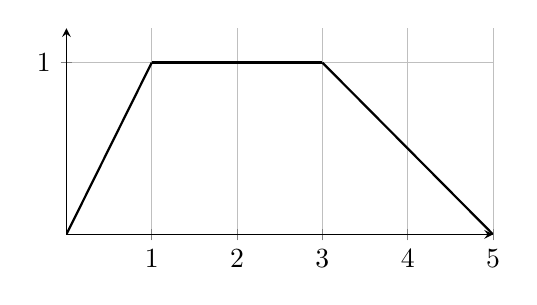
\begin{tikzpicture}
\begin{axis}[
  width=7cm,height=4.2cm,
  axis lines=middle, grid=both,
  xmin=0, xmax=5, ymin=0, ymax=1.2,
  xtick={0,1,2,3,4,5}, ytick={0,1},
]
  \addplot[thick] coordinates {(0,0) (1,1)};
  \addplot[thick] coordinates {(1,1) (3,1)};
  \addplot[thick] coordinates {(3,1) (5,0)};
\end{axis}
\end{tikzpicture}
\task 


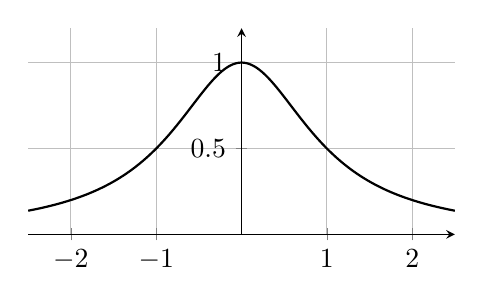
\begin{tikzpicture}
\begin{axis}[
  width=7cm,height=4.2cm,
  axis lines=middle, grid=both,
  xmin=-2.5, xmax=2.5, ymin=0, ymax=1.2,
  xtick={-2,-1,0,1,2}, ytick={0,0.5,1},
]
  \addplot[domain=-2.5:2.5, samples=300, thick]
    {1/(1 + x^2)};
\end{axis}
\end{tikzpicture}

\task 


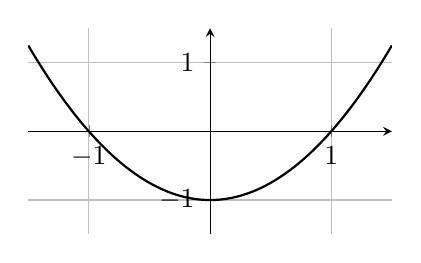
\begin{tikzpicture}
\begin{axis}[
  width=6.2cm,height=4.2cm,
  axis lines=middle, grid=both,
  xmin=-1.5, xmax=1.5, ymin=-1.5, ymax=1.5,
  xtick={-1,0,1}, ytick={-1,0,1},
]
  \addplot[domain=-1.5:1.5, samples=200, thick]
    {x^2 - 1};
\end{axis}
\end{tikzpicture}


\task 


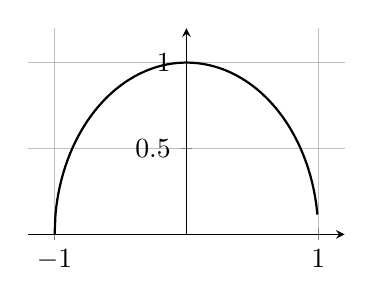
\begin{tikzpicture}
\begin{axis}[
  width=5.6cm,height=4.2cm,
  axis lines=middle, grid=both,
  xmin=-1.2, xmax=1.2, ymin=0, ymax=1.2,
  xtick={-1,0,1}, ytick={0,0.5,1},
]
  \addplot[domain=-1:1, samples=300, thick]
    {sqrt(1 - x^2)};
\end{axis}
\end{tikzpicture}
\end{tasks}
}
\correction{
\tcblower
{\scriptsize \textit{Correction générée par IA}}

Pour esquisser le graphe de $f'$, on observe la pente de $f$ en chaque point.

\begin{tasks}(2)
\task
La fonction $f$ est composée de trois segments~:
\begin{itemize}
\item Sur $\interval{0}{1}$~: la pente est constante et égale à $1$, donc $f'(x)=1$.
\item Sur $\interval{1}{3}$~: la fonction est constante, donc $f'(x)=0$.
\item Sur $\interval{3}{5}$~: la pente est constante et égale à $\dfrac{0-1}{5-3}=-\dfrac{1}{2}$, donc $f'(x)=-\dfrac{1}{2}$.
\end{itemize}
En $x=1$ et $x=3$, la fonction $f$ n'est pas dérivable (changements brusques de pente).

Le graphe de $f'$ est donc~: $f'(x)=1$ sur $]0,1[$, $f'(x)=0$ sur $]1,3[$, et $f'(x)=-\dfrac{1}{2}$ sur $]3,5[$.

\task
La fonction $f(x)=\dfrac{1}{1+x^2}$ a la forme d'une cloche symétrique par rapport à l'axe des ordonnées.
\begin{itemize}
\item $f'(x)=0$ en $x=0$ (maximum de $f$).
\item $f'(x)<0$ pour $x>0$ (fonction décroissante).
\item $f'(x)>0$ pour $x<0$ (fonction croissante).
\end{itemize}
Le graphe de $f'$ passe par l'origine, est positif pour $x<0$, négatif pour $x>0$, et symétrique par rapport à l'origine (fonction impaire).

\task
La fonction $f(x)=x^2-1$ est une parabole.
\begin{itemize}
\item $f'(x)=2x$ est une droite passant par l'origine.
\item En $x=0$, la tangente à la parabole est horizontale, donc $f'(0)=0$.
\item Pour $x>0$, la pente est positive et croissante.
\item Pour $x<0$, la pente est négative et décroissante.
\end{itemize}
Le graphe de $f'$ est une droite $y=2x$.

\task
La fonction $f(x)=\sqrt{1-x^2}$ représente un demi-cercle.
\begin{itemize}
\item En $x=0$, la tangente est horizontale, donc $f'(0)=0$.
\item Lorsque $x$ s'approche de $-1$ ou $1$, la tangente devient verticale, donc $f'(x)\to \pm\infty$.
\item $f'(x)<0$ pour $x>0$ (fonction décroissante).
\item $f'(x)>0$ pour $x<0$ (fonction croissante).
\end{itemize}
Le graphe de $f'$ passe par l'origine, avec des asymptotes verticales en $x=-1$ et $x=1$.
\end{tasks}
}
